\chapter{Passive Dynamics of Legged Locomotion}
\label{sec:PassiveDynamicsOfLeggedLocomotion}
\index{passive dynamics}

In section \ref{sec:SLIP} it was said that the SLIP locomotive could achieve
stable motion if initial conditions are appropriate. The fact that such motion
can sustain itself without any active feedback or input (an isolated system)
means the motion is passively stable. Thus, it may be possible to achieve
locomotion passively. This has various implications, especially for the design
of efficient (and thus more human-like) walking robots \cite{collins}. To build
up to an analysis of passive SLIP motion, we first examine the passive 2D
motion of a rimless wheel rolling down an incline.


%%%%%%%%%%%%%%%%%%%%%%%%%%%%%%%%%%%%%%%%%%%%%

% I just put this section here from the "introduction to stability" It may be spread around to other places. 

\section{Introduction to Stability} % (notes page 20-26)
\label{sec:IntroductionToStability}
\index{stability}

Understanding the passive dynamics of the models presented in Chapter
\ref{sec:ModelingLeggedLocomotion} requires a basic understanding of the
concept of stability. We consider locomotion to be a stable periodic motion of
a dynamic system, where the dynamic system is defined by ordinary differential
equations and sometimes collision equations. The motion of a dynamic system is
considered to be stable when the system is capable of rejecting disturbances.
A legged animal or robot that is moving with a stable gait, given some
perturbation in its motion, will return to the motion it was performing before
the perturbation was introduced. Experiment and theory have both shown that
certain legged animals and robots can walk or run with a stable motion without
any control; the motion is passively stable. We will see later on that the
mathematical description for such motion is a stable fixed point on a Poincare
section or map. 

% FIGURE
\begin{figure}[h]		% h="here" t="top" b="bottom" p="separate page"
\begin{centering}
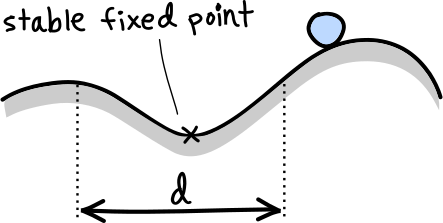
\includegraphics[width=0.55\textwidth]{Figures/BallOnHill}\par
\end{centering}
\caption[Diagram: Ball in a Valley]{Ball in a valley. If the ball is released
from the hill to the right at a height that is no greater than that of the hill
to the left, the ball will remain in the valley between hills. After some time,
the ball comes to rest at the stable fixed point at the bottom of the valley.
The steady state position of the ball can also be thought of as periodic motion
in which the ball is found at the stable fixed point at the end of each period
of the motion. This periodic motion mindset is useful for locomotion models.}
\label{fig:BallOnHill}
\end{figure}
%

Imagine a system like the one shown in figure \ref{fig:BallOnHill}: two hills,
with a valley between them, and a ball that starts on the side of the larger
hill. Imagine that the interaction between the ball and the hill is \emph{not}
frictionless, but the rolling resistance is small. When the ball is released,
it rolls left down the hill, passing by the lowest point in the valley,
and rolls over the peak of the smaller hill. Now imagine the ball starts a
little bit lower on the side of the larger hill, such that it rolls through the
valley, and does not roll past the peak of the smaller hill. It reaches some
maximum height, and rolls back the way it came. The ball oscillates back and
forth until it comes to rest at the bottom of the valley. 

Though slightly un-intuitive, one can think of the motion of the ball as
periodic in time. When the ball is resting at the bottom, we consider the ball
to be in ``motion," where the period of the motion is infinitesimal. The
resting point is considered a stable fixed point, because for every period of
the motion, the ball returns to that point. If the ball's ``motion" is
disturbed by an external force, after some number of periods it will return to
the stable fixed point. In this case, it is a little silly to think of it that
way, because between periods, the ball is still at stable fixed point during
its ``motion." \todo{get rid of preceding sentence?} The path that it
follows along the hill as it settles to that fixed point can be thought of as
the basin of attraction: if the ball starts anywhere in the basin, it reaches
the stable fixed point. 

In the case of the ball in figure \ref{fig:BallOnHill}, the basin of attraction
is two-dimensional. The ball can be assumed to be on the surface of the hill,
and its state can be described by two parameters: position along the path, and
velocity in the direction of travel. A Poincare map is a visualization of these
two parameters sampled once per period, in two-dimensional space, as in figure
\ref{fig:BasinOfAttraction}. Parameters like position and velocity can be
assigned to the $x$ and $y$ axes of the Poincare map, and the stable fixed
point can be located on the map. Figure \ref{fig:BasinOfAttraction} is a
generalized version of a Poincare map. In the case of the ball on the hill, the
stable fixed point would be at position $y = 0$ and velocity $x = 0$. A general
fixed point is marked with a star on the map, as shown in figure \ref{fig:BasinOfAttraction}. 

% FIGURE
\begin{figure}[h]		% h="here" t="top" b="bottom" p="separate page"
\begin{centering}
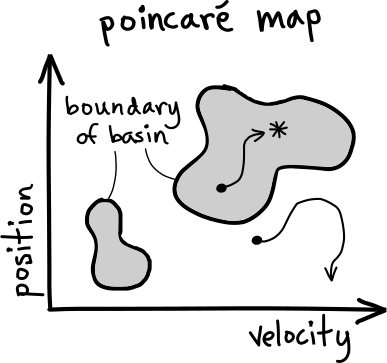
\includegraphics[width=0.3\textwidth]{Figures/BasinOfAttraction}\par
\end{centering}
\caption[Diagram: Poincare Map with Basins of Attraction]{Poincare map with basins of attraction. The map, drawn here for a general system, has coordinates of position and velocity. Points on the map denote the position and velocity state of a system at the end of each period of the system's motion. Basins of attraction are shaded, and fixed points are labeled as stars. If the initial state of a system, denoted as a dot, is within a basin of attraction, the system will tend toward the fixed point contained in that basin. If the initial state lies outside a basin, its configuration in time does not tend toward a particular steady motion.}
\label{fig:BasinOfAttraction}
\end{figure}
%

\todo{can there be a basin of attraction without a fixed point, as is
shown in the figure?}

The basin of attraction is made up of all the states (position and velocity)
that the system can have initially and still return to the stable fixed
point. In the ball example, it is important to note that the ball may start in
the region $d$ shown in figure \ref{fig:BallOnHill}, but if the velocity is
nonzero and too great, the ball may never reach the stable fixed point. 

\todo{change the previous sentence to ``if the velocity is
leftward, the ball will never reach the stable fixed point''?}

In general, it is possible to have part of the basin of attraction detached
form the part that contains the fixed point, as is shown in figure
\ref{fig:BasinOfAttraction}.

The stable fixed point is generally called an attractor, and up to this point
we have been thinking of the attractor as a single point on the Poincare map.
However, it is also possible that the attractor could be a complicated curve or
region. These complicated regions are sometimes called ``strange attractors."
Functionally, strange attractors are the same as a stable fixed point. If the
state of the system lies within the attractor, it will return to somewhere else
within that attractor one period later, just as a system would return to the
stable fixed point one period later. Figure \ref{fig:Attractors} shows the
difference between the two attractors.

% FIGURE
\begin{figure}[h]		% h="here" t="top" b="bottom" p="separate page"
\begin{centering}
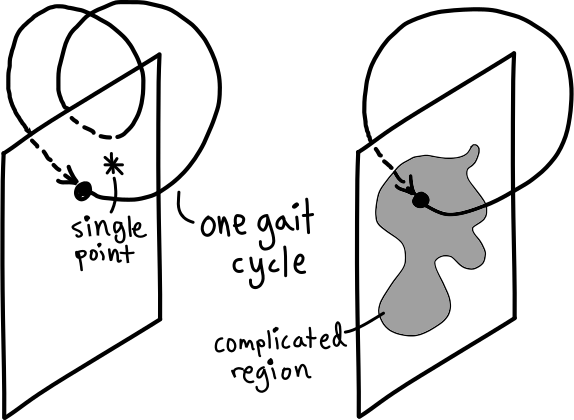
\includegraphics[width=0.5\textwidth]{Figures/Attractors}\par
\end{centering}
\caption[Diagram: Single Point Attractors and Strange Attractors]{Single point
attractors and strange attractors. The left Poincare section is for a single
point attractor, denoted by the star. The right Poincare section is for a
strange attractor, where the shaded area is the strange attractor. If the
system's state is within an attractor region, the system's state at the end of
each period will lie within the attractor. Note that the basin of attraction is
not shown for either attractor. The strange attractor on the right could be
enclosed by a larger basin of attraction. If a disturbance is introduced that
doesn't move the trajectory outside the basin of attraction, the trajectory
will return to the complicated region after some time.}
\label{fig:Attractors}
\end{figure}
%

\todo[inline]{I like how the loop shows a period. maybe axes again would help?
I don't know. Also this might be confusing since gray
was also used to show the basin of attraction in a previous figure. Also the
figure seems to indicate that for a strange attractor, for every period you do
come back to the same state.}

The section shown on the left of figure \ref{fig:Attractors} is an example of a
single point attractor, showing what might happen if a disturbance is
introduced. The trajectory traced around the section shows that the motions are
periodic, and do not quite pass through the stable fixed point on each period.
As long as the trajectory of the state passes through the basin of attraction,
the trajectory of the state will return to the stable fixed point, and become a
single loop like in the section shown on the right. 

As may be apparent from the previous two figures, much of our analysis of
stability is rooted in the state-space representation of systems. In such a
representation, there is a state at which the robot is operating. If we
introduce a disturbance to the state, perhaps $\epsilon$, we want to know if
the state space representation returns to what it was before the disturbance
was introduced. More tools for analyses like this can be found in books on
feedback control, such as Ogata \cite{ogata09} (Root Locus, Nyquist, etc).
These tools will not be used extensively in this chapter, but understanding the
reasons for their use in other systems will be helpful to understanding
stability analyses of legged locomotion models. 

%%%%%%%%%%%%%%%%%%%%%%%%%%%%%%%%%%%%%%%%%%%%

\section{Rimless Wheel} % (notes page 20-26)
\label{sec:RimlessWheel}
\index{rimless wheel dynamics}

The motion of a rimless wheel is a classical problem that exhibits some basic
aspects of passive stable motion and permits a nice introduction to examining
the stability of locomotion models. Consider the rimless wheel in figure
\ref{fig:RimlessWheel}, with massless spokes and a mass $m$ at its center, that
is rolling down an incline $\gamma$ under the force of gravity along $\ul$. The
wheel has $N$ spokes of length $l$, and each spoke is separated from the next
by the angle $\phi$. The moment of inertia of the wheel about its center $G$ is
$I$. The angle between the incline's normal and the spoke that is in contact
with the incline is $\theta = \theta(t)$. The wheel pivots without slip about
the end of this spoke, at point $C$. While pivoting, the wheel's center of mass
undergoes a motion that can be described as \textit{unstable falling}
\cite{coleman96}. This smooth motion occurs in between the plastic collisions
of the spokes with the incline.

% FIGURE
\begin{figure}[h]		% h="here" t="top" b="bottom" p="separate page"
\begin{centering}
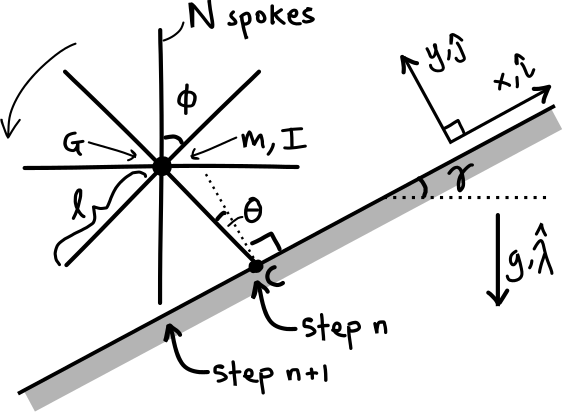
\includegraphics[width=0.6\textwidth]{Figures/RimlessWheel}\par
\end{centering}
\caption[Diagram: Rimless Wheel]{Rimless wheel. A rimless spoked wheel rotates
down an incline with slope $\gamma$. The $N$ massless spokes of length $l$ are
separated equally by the angle $\phi$ . The mass $m$ is located at the center of
the wheel, and the wheel has moment of inertia $I$. The orientation of the
wheel is specified by the angle $\theta$ that the spoke contacting the incline
makes with the incline's normal.}
\label{fig:RimlessWheel}
\end{figure}
%

Our objective with the rimless wheel is to compute its motion, given the
parameters above, and to examine its stability. The motion has two portions:
smooth motion and collisions.  The motion is most likely (but not necessarily)
periodic, so these two portions repeat again and again. Under the right
conditions, the wheel is able to achieve stable motion without any active
control.

\textbf{Smooth ``flight":} The velocity of the mass is continuous between
collisions. Angular momentum balance is a natural choice for finding the
motion, since angular momentum balance about point $C$ avoids the
undesired unknown of the reaction force at $C$. Using the free body diagram in
figure \ref{fig:RimlessSmoothAndCollision}a,

\begin{align}
\Sigma \vec{\mathbf{M}}_{/C} &= \dot{\vec{\mathbf{H}}}_{/C} \notag \\
l \hat{\mathbf{e}}_r \times mg \ul &= \vec{\mathbf{r}}_{G/C} \times m\vec{\mathbf{a}}_G + I \dot{\omega} \hat{\mathbf{k}}
\label{eq:RimlessAMB}
\end{align}

where $\hat{\mathbf{e}}_{r}$ is a unit vector pointing from the contact point $C$ to the center of mass of the wheel $G$. The unit vectors in equation \ref{eq:RimlessAMB} can be written explicitly, and the acceleration can be written in polar coordinates.

\begin{align}
\hat{\mathbf{e}}_{r} &= - \sin{\theta} \ui + \cos{\theta} \uj \\
\ul &=  - \sin{\gamma} \ui - \cos{\gamma} \uj \\
\va_{G} &= l \thetaddot \ueth - l \thetadot^{2} \uer
\end{align}

After substituting these expressions into equation \ref{eq:RimlessAMB}, employing the trigonometric sine sum identity and performing some additional algebra, we arrive at a system of two first-order nonlinear differential equations that can be solved perhaps with a computer solver.

\begin{align}
\dot{\theta} &= \omega \label{eq:RimlessODE2} \\
\dot{\omega} &= \frac{mgl}{I + m l^2} \sin(\theta + \gamma) \label{eq:RimlessODE1}
\end{align}

This equation of motion is very similar to that of an inverted pendulum,
considering that the coefficient in equation \ref{eq:RimlessODE1} is constant,
and that $\gamma$ is constant as well. As with any differential equation in
time, its solution requires initial conditions. The rotation of the wheel
initially is $\theta_{0} = \theta_n^{+}$, the rotation at the end of the $n$-th
collision. We choose this to be $-\phi/2$ because the end of the collision is
ambiguous. The angular speed at the start of the ``flight'' is $\omega_{0} =
\omega_{n}^{+}$, the angular speed of the wheel after the $n$-th collision. For
the first flight, this value is simply chosen. For subsequent motion, this
value comes from the spoke collision calculation for the $n$-th collision. To
obtain this, we must examine the spoke collision.

\textbf{Spoke collision:} Initial conditions for the angular speed \emph{after} the first ``flight'' are required to solve equations \ref{eq:RimlessODE2} and \ref{eq:RimlessODE1}. The initial position $\theta_{n+1,0}$ is always set as $\phi/2$, but the initial angular speed $\omega_{n+1,0}$ takes on the the angular speed at the end of the $n$+1-th collision, $\omega_{n+1}^{+}$. It is the objective of this spoke collision calculation to determine $\omega_{n+1}^{+}$ from the angular speed before the collision $\omega_{n+1}^{-}$. This relationship is found from conservation of angular momentum about point $C$ when the wheel is in the configuration shown in figure \ref{fig:RimlessSmoothAndCollision}b.

\begin{align}
\vec{\mathbf{H}}_{/C,n+1}^{-} &= \vec{\mathbf{H}}_{/C,n+1}^{+}
\label{eq:RimlessAM}
\end{align}

If there are no external torques about the point about which the angular momenum is calculated, then the angular momentum direclty before and directly after the collision must be the same. The only force that could cause a moment about the pivot point $C$ is the weight of the center of the wheel. However, the collision occurs over a short enough time period that the weight can be ignored. Again, the contact impulse at point $C$ does not contribute to the angular momentum about point $C$.

% FIGURE
\begin{figure}[h]		% h="here" t="top" b="bottom" p="separate page"
\begin{centering}
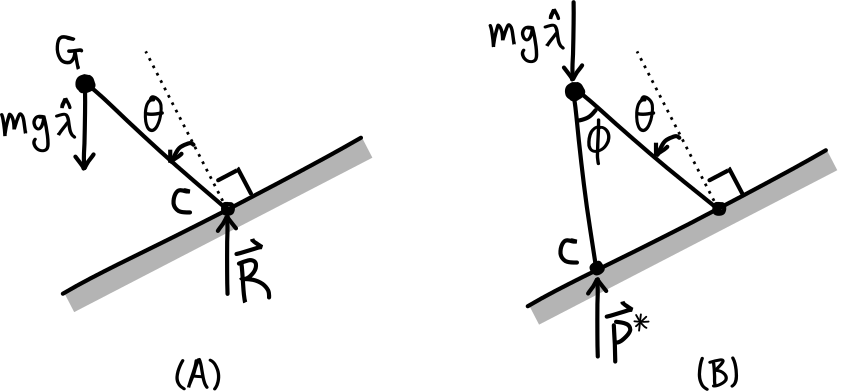
\includegraphics[width=0.7\textwidth]{Figures/RimlessSmoothAndCollision}\par
\end{centering}
\caption[Diagram: Rimless Wheel Free Body Diagrams]{Rimless wheel free body diagrams. Diagram (A) is a free body diagram for the smooth ``flight'' of the wheel. Diagram (B) is a free body diagram for the spoke collision of the wheel.}
\label{fig:RimlessSmoothAndCollision}
\end{figure}
%

The angular momentum before collision $n+1$ is

\begin{equation}
\vec{\mathbf{H}}_{/C,n+1}^{-} = \vec{\mathbf{r}}_{G/C} \times m\vec{\mathbf{v}}_{G}^{-} + I \omega_{n+1}^{-} \vec{\mathbf{k}}
\label{eq:RimlessHMinus}
\end{equation}

The angular momentum after collision $n+1$ is

\begin{equation}
\vec{\mathbf{H}}_{/C,n+1}^{+} = (I + ml^{2} ) \omega_{n+1}^{+} \hat{\mathbf{k}}
\label{eq:RimlessHPlus}
\end{equation}

Here, the moment of inertia used is about point $C$. Accordingly, this moment of inertia is the sum of the centroidal moment of inertia and a term from the parallel axis formula. By equating these two momenta and expressing explicity all the terms in equation \ref{eq:RimlessHMinus}, the angular speed after the collision is given by

\begin{equation}
\omega_{n+1}^{+} = \frac{I + ml^{2} \cos{\phi}}{I + ml^2} \omega_{n+1}^{-}
\label{eq:RimlessOmegaPlus}
\end{equation}

We see that the angular speed changes by a factor that depends only on the mass
and geometry of the wheel.

Now that we have our initial conditions for the smooth flight. we can piece
together the ``flight'' and collision. A qualitative description of the rimless
wheel motion is given by the graphs in figure \ref{fig:RimlessPlots}. Collision
$n$ ends at $t = 0$ and collision $n+1$ starts at $t = t^*$. The wheel rotates
quickly with $\omega = \omega_{n}^{+}$ right after the collision. Depending on
$\phi$, the mass may start its smooth ``flight'' motion before or \emph{at} the
apex of its ``flight'' path. If $\phi$ is sufficiently large, the mass slows
down as its mass is elevated to the apex of the path. If not, the mass starts
its ``flight'' at the apex.  The minimum angular speed is achieved at the apex
of the smooth "flight". The wheel accelerates downward from its apex as the
next spoke approaches collision. Just before the collision, the wheel rotates
with angular speed $\omega = \omega_{n+1}^{-}$ (figure
\ref{fig:RimlessPlots}b).

% FIGURE
\begin{figure}[h]		% h="here" t="top" b="bottom" p="separate page"
\begin{centering}
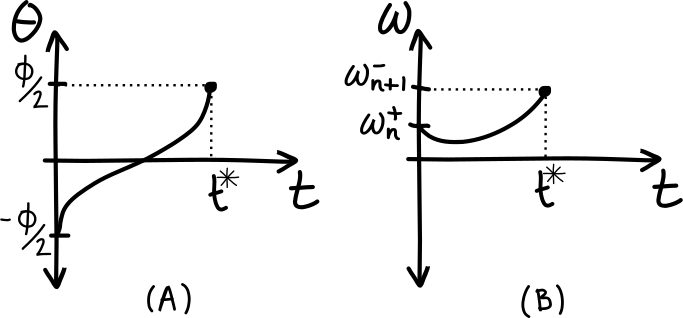
\includegraphics[width=0.7\textwidth]{Figures/RimlessPlots}\par
\end{centering}
\caption[Plot: Rimless Wheel State vs. Time for Smooth ``Flight'']{Rimless
wheel state vs. time for smooth flight. Plot (A) shows the rotation of the
wheel throughout the smooth ``flight'', up until the time $t^{*}$ when the
collision occurs. The flight is defined as occuring between $\theta = -\phi/2$
and $\theta = \phi/2$. Plot (B) shows the angular speed throughout the smooth
``flight'', which starts at $\omega_{n}^{+}$ and ends at $\omega_{n+1}^{-}$.}
\label{fig:RimlessPlots}
\end{figure}
%
\begin{comment}
 The dip in the curve depends on the the spoke separation $\phi$.
\end{comment}

% FIGURE
\begin{figure}[h]		% h="here" t="top" b="bottom" p="separate page"
\begin{centering}
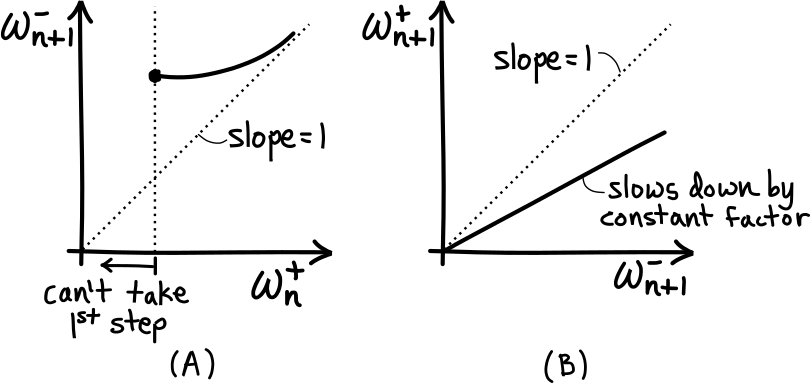
\includegraphics[width=0.7\textwidth]{Figures/RimlessPlots2}\par
\end{centering}
\caption[Plot: Rimless Wheel Angular Speed Relations]{Rimless wheel angular speed relations. Plot (A) provides $\omega_{n+1}^{-}$ at the end of the ``flight'' from $\omega_{n}^{+}$ from the beginning of the ``flight''. Plot (B) provides the angular speed after the collision $\omega_{n+1}^{+}$ from the angular speed before the collision $\omega_{n+1}^{-}$.}
\label{fig:RimlessPlots2}
\end{figure}
%
\begin{comment}
The curve asymptotically approaches $\omega_{n+1}^{-} = \omega_{n}^{+}$ as gravity has less time to accelerate the wheel for faster initial angular speeds. 
\end{comment}

The periodic evolution of the wheel's angular speed before and after collisions
is described by figure \ref{fig:RimlessPlots2}. Figure \ref{fig:RimlessPlots2}a
describes the change in angular speed between the beginning and end of the
smooth flight. There is a threshold value below which continued motion is not
possible and the wheel does not proceed continually down the incline. In this
case the wheel does not have enough momentum after the collision to move
through the apex of the smooth flight path. For greater initial speeds
$\omega_{n}^{+}$, the wheel starts the smooth flight with more momentum and
thus finishes the flight with a greater final speed $\omega_{n+1}^{-}$. The
curvature in this relation results from the fact that the force of gravity
contributes less to the increased final speed for higher values of the initial
speed. For large $\omega_{n}^{+}$ the flight occurs quickly enough that the
downward acceleration due to gravity does not have the time to noticably
increase the speed of the wheel.

Figure \ref{fig:RimlessPlots2}b picks up where figure \ref{fig:RimlessPlots2}a
leaves off, literally. This figure provides the difference between the speed
$\omega_{n+1}^{-}$ before the subsequent collision and the speed
$\omega_{n+1}^{+}$ after the subsequent collision.  \todo{The angular speed of
the wheel is discontinuous through the collision since the collision is not
elastic. chris: i now think the collision is elastic} The slope of the straight
line in figure \ref{fig:RimlessPlots2}b is given by the constant factor in
equation \ref{eq:RimlessHPlus}. The slope here can be thought of as a
coefficient of restitution.

\begin{comment}
Keep in mind that the curves in these plots are dependent on the parameters of
the rimless wheel model. For example, if $\gamma = 0$ then the incline becomes
a flat surface and the motion is not as interesting as for the general case
examined here. \todo[inline]{Chris: remove?: If $\gamma = 0$, the motion cannot
be stable if the collisions are not perfectly elastic.}
\end{comment}

% FIGURE
\begin{figure}[h]		% h="here" t="top" b="bottom" p="separate page"
\begin{centering}
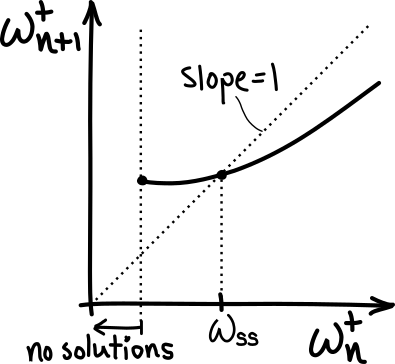
\includegraphics[width=0.3\textwidth]{Figures/RimlessStrideFunction}\par
\end{centering}
\caption[Plot: Rimless Wheel Stride Function]{Rimless wheel stride function. Provides the angular speed at the start of a ``flight'' from the angular speed at the start of the previous ``flight''. This figure is generated from a composition of the plots in figure \ref{fig:RimlessPlots2}. The point at which the curve intersects the $\omega_{n+1}^{+} = \omega_{n}^{+}$ line is a stable fixed point.}
\label{fig:RimlessStrideFunction}
\end{figure}
%

We now consider the stability of the rimless wheel. The composition of the
graphs in figure \ref{fig:RimlessPlots2} yields figure
\ref{fig:RimlessStrideFunction}, which is called a \emph{stride
function}\index{stride function}. The stride function can be used to understand
how the motion of the wheel evolves over numerous collisions. To determine the
motion of the wheel, or $\omega_{n+1}$, throughout multiple cycles of its
motion, use the following procedure with figure
\ref{fig:RimlessStrideFunction}:

\begin{enumerate}
\item Choose an initial value $\omega_{0}^{+}$ on the $\omega_{n}^{+}$-axis.
\item Trace this point up to the thick curve. This point on the thick curve provides the value of $\omega_{1}^{+}$ on the vertical axis.
\item Now $n = 1$; find the value of $\omega_{1}^{+}$ on the horizontal axis by
    tracing horizontally to the \textit{slope = 1} line.
\item Trace vertically from the \textit{slope = 1} line to the thick line to discover the value of $\omega_{2}^{+}$ on the vertical axis.
\item Repeat.
\end{enumerate}

\todo[inline]{Chris: I'd say we should put in a basin of attraction plot here
but am I right that we cannot do so, since, there is only one variable, that
determines stability?}

Again, the angular speed at the beginning of the smooth flight must surpass a
threshold value. If the initial angular speed in a given period has the steady
state value $\omega_{ss}$, then the subsequent motion is steady and periodic
until the wheel is perturbed. Note that the threshold angular speed, the steady
state angular speed, and the shape of the curve in the figure are all functions
of the model's parameters. Since the curve is increasing everywhere, all values
of $\omega_n^+$ above the threshold cause $\omega_n^+$ (and $\omega_{n+1}^{+}$)
to tend toward $\omega_{ss}$. That is, this system always tends toward the
stable fixed point $\omega_{ss}$ for the parameters used for figure
\ref{fig:RimlessStrideFunction}.

\section{Spring Loaded Inverted Pendulum} %(notes page 27-30)
\label{sec:SpringLoadedInvertedPendulum}

We now return to the SLIP model presented in section \ref{sec:SLIP} and analyze
its passive stability. In order to do so, we must first give careful thought to
the construction of its Poincare map.

Remember that the Poincare map is constructed by sampling the variables that
describe the motion of the system once per period, and plotting those points.
Therefore, we must assume that the model travels with a periodic gait. For the
SLIP model of walking and running, the system's state can be fully described by
four state variables related to the model's center of mass: $x$, $y$,
$\dot{x}$, and $\dot{y}$. The contact angle of the leg, $\theta_{c}$, is
considered to be an initial condition, and is not a part of the system state.

The point at which one ``slices'' the gait cycle is called a Poincare section,
and we must choose a section for our map. Our choice of section affects the
number of equations which we must solve to fully define the motion of the
hopper. We hope to choose a section that minimizes the number of equations.
Also, a Poincare map of a system ideally uses only two state variables.
However, this may not always be possible.  There are quite a few options for
points along the SLIP gait cycle to construct a Poincare map. There are peaks
and valleys in the gait trajectory of the center of mass of the model, as shown
in figure \ref{fig:SLIPSections}.   Six possible sections are:

\begin{enumerate}

\item Transition from stance to flight. Choosing this transition point allows
    the gait trajectory to be built from only two segments: a stance phase and
    a parabolic flight phase. \todo{how many section variables?}

\item Transition from flight to stance. No need to worry about
    $y=l_{0}\cos{\theta_{c}}$. \todo{what?} Three section state variables: $x$, $\dot{x}$, and
    $\dot{y}$.

\item Point of maximum height in flight: $\dot{y}=0$. Three section state variables: $x$, $\dot{x}$, and $y$.
\label{item:MaxHeight}

\item Point of minimum height in stance: $\dot{y}=0$. Three section state variables: $x$, $\dot{x}$, and $y$.

\item Point where the spring is maximally compressed.

\item Point where the stance leg is vertical.

\end{enumerate}

% FIGURE
\begin{figure}[h]		% h="here" t="top" b="bottom" p="separate page"
\begin{centering}
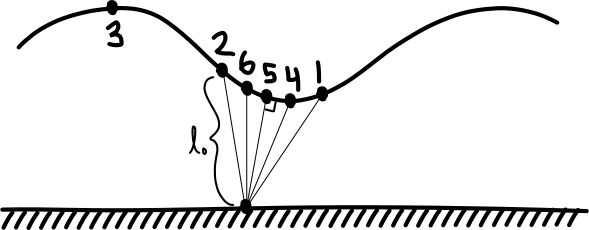
\includegraphics[width=0.6\textwidth]{Figures/SLIPSections}\par
\end{centering}
\caption[Diagram: SLIP Options for Poincare Sections]{SLIP options for Poincare sections. Various points in the gait cycle of the SLIP model can be used to generate a Poincare map. The section, or a particular slice of the periodic gait cycle, can fully define the motion. Each section is defined by a different occurence. Six different options are proposed, and option 3 is considered in more detail.}
\label{fig:SLIPSections}
\end{figure}
%

Though all of the options are valid, section \ref{item:MaxHeight} will be
analyzed here in further detail. This section reduces the four-dimensional
phase space using $x$, $y$, $\dot{x}$, and $\dot{y}$ to a three-dimensional
state space using only $x$, $\dot{x}$, and $y$ because it is known that
$\dot{y} = 0$ at the section slice. Additionally, we do not need to know $x$ in
order to predict the motion of the center of mass because the center of mass is
traveling only in the $x$ direction, and its location relative to the $x$-axis
is irrelevant if the motion is periodic. Getting rid of $x$ reduces our state
space to two dimensions. Given $y_{n}$ and $\dot{x}_{n}$, we want to predict
$y_{n+1}$ and $x_{n+1}$, where $n$ is an index through sequential
sections of the periodic motion.

Given the model and the free body diagram presented in section \ref{sec:SLIP},
we can calculate the trajectory of the center of mass. Such knowledge will
allow us to analyze the stability of SLIP motion. We can the trajectory with a
numerical ordinary differential equation (ODE) solver. Two such solvers are
MATLAB's ODE45 and ODE112. For the remainder of this section, we will describe
the simulation of the SLIP model in the context of MATLAB.

The SLIP model features three distinct segments of motion for the chosen
Poincare section. The first is the parabolic flight from the top of the
trajectory to where the leg initially touches the ground. This first segment of
motion is described by one set of differential equations. The second segment of
motion is the stance phase, in which the leg contacts the ground and the spring
is compressed. This segment is described by a different set of differential
equations. Finally, the third segment is again parabolic flight, described by
the same differential equations as the first segment. The transition between
the segments of motion can often be detected with an event detection feature of
the ODE solver, as is the case in MATLAB.

\begin{comment}
In the world of legged locomotion, it is important to analyze the stability of
locomotion models.
\end{comment}

Equipped with a choice for a Poincare section, we are almost ready to analyze
the passive stability of the SLIP model. We first require a stride function, or
return map, that describes how the center of mass changes state from $y_{n}$
and $\dot{x}_{n}$ to $y_{n+1}$ and $\dot{x}_{n+1}$.  For clarity in this
analysis, we define $q_{1}\equiv y_{n}$ and $q_{2}\equiv\dot{x}_{n}$. We also
define $\mathbf{q}$ as a vector of the two states $q_{1}$ and $q_{2}$, The
vector $\mathbf{q}_{n+1}$ is a function of $\mathbf{q}$, and so we define
$\mathbf{q}_{n+1} = \mathbf{f}(\mathbf{q})$.  We split the vector function
$\mathbf{f}(\mathbf{q})$ into two scalar functions, one for each state variable.

\begin{align}
q_{1,n+1}= f_{1}(q_{1,n},q_{2,n}) \notag \\
q_{2,n+1}=  f_{2}(q_{1,n},q_{2,n})
\label{eq:FullFunctionDefinition}
\end{align}

For a given $\mathbf{q}_{n}=[q_{1,n},q_{2,n}]^{T}$, the fixed point that
describes periodic motion occurs when
$\mathbf{q}_{n+1}=\mathbf{f}(\mathbf{q}_{n})=\mathbf{q}_{n}$. This fixed point
can be found using a method similar to that used to find the fixed point for
the motion of the rimless wheel. However for this problem, the calculations
will be performed in two dimensions, not one.

Given some kind of simulation that uses MATLAB's ODE solvers to calculate the
trajectory of the center of mass, We can obtain values for $q_{n}$ and
$q_{n+1}$ by simulating the motion using an ODE solver, as described above.
This provides us with an implicit definition of the function $\mathbf{f}$,
seeing as the ODE solver provides $\mathbf{q}_{n+1}$ from $\mathbf{q}_n$.
Equipped with $\mathbf{f}$, we can solve for the fixed point of the system
using a numerical nonlinear root-finder, such as MATLAB's FSOLVE.  However,
roofinders require that the problem takes the form $\mathbf{g}(\mathbf{q})=0$,
so we define a function $\mathbf{g}(\mathbf{q}) \equiv
\mathbf{f}(\mathbf{q})-\mathbf{q}$. To obtain periodic motion, the goal is to
solve for $\mathbf{q}$ such that $\mathbf{g}(\mathbf{q})=0$. This solution is
called the ``root'' and will be referred to here as $\mathbf{q}^{*}$.

 \begin{align}
 \begin{bmatrix}
 f_{1}(q_{1},q_{2}) \\
 f_{2}(q_{1},q_{2})
 \end{bmatrix}
 -
 \begin{bmatrix}
 q_{1} \\
 q_{2}
 \end{bmatrix}
 =
 \begin{bmatrix}
 0 \\
 0
\end{bmatrix}
\label{eq:GDefinition}
\end{align}


After solving equation \ref{eq:GDefinition}, it is desirable to know if the
motion is stable near this fixed point. To assess the stability of the fixed
point $\mathbf{q}^{*}$, the function $\mathbf{f}(\mathbf{q})$, must first be
linearized about $\mathbf{q}^{*}$.  This can be done with the first two terms
of a Taylor expansion:

\begin{equation}
    \mathbf{f} ( \mathbf{q} ) = \mathbf{f} ( \mathbf{q}^{*} ) +
    \frac{d}{d\mathbf{q}}\mathbf{f} (\mathbf{q}^{*}) ( \mathbf{q}
    - \mathbf{q}^{*} )
\label{eq:LinearShorthand}
\end{equation}

If the function $\mathbf{f}(\mathbf{q})$ is expanded, a matrix called the
Jacobian, $\mathbf{J}$, reveals itself. By examining the expanded form of the
Taylor approximation of $\mathbf{f}(\mathbf{q})$, it is easy to see why the
Jacobian determines the stability of the motion described by
$\mathbf{f}(\mathbf{q})$:

\begin{align}
\begin{bmatrix}
f_{1} (q_{1},q_{2}) \\
f_{2} (q_{1},q_{2}) 
\end{bmatrix}
=
\begin{bmatrix}
q_{1}^{*} \\
q_{2}^{*}
\end{bmatrix}
+
\begin{bmatrix}
\displaystyle\frac{\partial f_{1}}{\partial q_{1}} &  \displaystyle\frac{\partial f_{1}}{\partial q_{2}} \\
\displaystyle \frac{\partial f_{2}}{\partial q_{1}} & \displaystyle \frac{\partial f_{2}}{\partial q_{2}}
\end{bmatrix}
\begin{bmatrix}
\epsilon_{1} \\
\epsilon_{2}
\end{bmatrix}
\label{eq:LinearLonghand}
\end{align}

We define the Jacobian as

\begin{equation}
    \mathbf{J} = 
\begin{bmatrix}
\displaystyle\frac{\partial f_{1}}{\partial q_{1}} &  \displaystyle\frac{\partial f_{1}}{\partial q_{2}} \\
\displaystyle \frac{\partial f_{2}}{\partial q_{1}} & \displaystyle \frac{\partial f_{2}}{\partial q_{2}}
\end{bmatrix}
\label{eq:Jacobian}
\end{equation}



For the motion to be periodic, it has already been shown that
$\mathbf{f}(\mathbf{q})$ must equal $\mathbf{q}^{*}$. Any time a given step
$\mathbf{q}$ is given as input to the return map $\mathbf{f}(\mathbf{q})$, the
return map must output the input.  The $\mathbf{q}$ that accomplishes this is
called $\mathbf{q}^{*}$ by definition. If the input $\mathbf{q}$ deviates from
this ideal $\mathbf{q}^{*}$ and causes $\mathbf{f}(\mathbf{q})$ to output
something other than the input $\mathbf{q}$, the motion is considered stable if
the system eventually returns the ideal $\mathbf{q}^{*}$ after a few periods.

This can be seen by examining the second term on the right side of equation
\ref{eq:LinearLonghand}, where $\epsilon_{1}$ is the error associated with
$q_{1}$ and $\epsilon_{2}$ is the error associated with $q_{2}$. These errors
$\epsilon_{1}$ and $\epsilon_{2}$ represent a disturbance introduced by
variation in the terrain or environment of the hopping robot. Every time the
robot goes through one gait cycle, the errors $\mathbf{\epsilon}$ will change
from some initial disturbance $\mathbf{\epsilon}_{0}$, based on the difference
between \todo{epsilon bold is not working out!!} the fixed point
$\mathbf{\mathbf{q}}^{*}$ and the output $\mathbf{f}(\mathbf{q})$, and the
values of the elements in the Jacobian, $\mathbf{J}$.
\todo{this previous sentence can still be made a little clearer I think}
\todo{how is the Jacobian calculated? I guess from the physical equations?}

Though the values of the elements of the Jacobian do not change with each step
(or period), the change in the errors $\mathbf{\epsilon}$ causes the value of
the second term of the right side of equation \ref{eq:LinearLonghand} to either
shrink or grow with each step. Whethe the error shrinks or grows depends on
$\mathbf{J}$. If the errors $\mathbf{\epsilon}$ grow, so does the second term
of the right side of equation \ref{eq:LinearLonghand}, and the motion of the
hopper is unstable. So the important question is: does the initial perturbation
$\mathbf{\epsilon}_{0}$ grow? This can be determined by examining the
product of the Jacobian and the perturbation vector $\mathbf{\epsilon}_{n}$:

\begin{align}
\begin{bmatrix}
\epsilon_{1,n+1} \\
\epsilon_{2,n+1}
\end{bmatrix}
=
%\begin{bmatrix}
%J_{11} &  J_{12} \\
%J_{21} &  J_{22} 
%\end{bmatrix}
\mathbf{J}
\begin{bmatrix}
\epsilon_{1,n} \\
\epsilon_{2,n}
\end{bmatrix}
\label{eq:ErrorAndJacobian}
\end{align}

\todo[inline]{I changed an equation here quite a bit, replacing the 2x2 J with
just the matrix symbol for the Jacobian. This might make this section harder to
read cursorily quickly}

\begin{comment}
In equation \ref{eq:ErrorAndJacobian} the subscripts denote the associated
element of $\mathbf{f}(\mathbf{q})$.
\end{comment}

In the following analysis, subscripts denote the step in the simulation. It is
clear that $\mathbf{\epsilon}_{1} = \mathbf{J}\mathbf{\epsilon}_{0}$ and
$\mathbf{\epsilon}_{2} = \mathbf{J}\mathbf{\epsilon}_{1} =
\mathbf{J}\mathbf{J}\mathbf{\epsilon}_{0}$.  It follows then that
$\mathbf{\epsilon}_{n} = \mathbf{J}\mathbf{\epsilon}_{n-1} =
\mathbf{J}^{n}\mathbf{\epsilon}_{0}$.  The goal here is to discover if
$\mathbf{\epsilon}_{n}$ decays to zero as $n$ reaches infinity.  If that is
true, then the hopper is stable. By making use of the eigenvector definition,
the value of $\mathbf{\epsilon}_{n}$ as $n$ reaches infinity can be found:

\begin{equation*}
    J \mathbf{v} = \lambda \mathbf{v}
\end{equation*}

Given that for this problem, $\mathbf{J}$ is a $2 \times 2$ matrix, there are
two eigenvalues $\lambda_i$ and two corresponding eigenvectors $\mathbf{v}_i$
that satisfy the eigenvector definition:

\todo[inline]{We have an issue here with subscripts! I'm not sure how to
resolve this right now\ldots}

\begin{align*}
    \mathbf{J} \mathbf{\epsilon} =& \mathbf{J} (a_{1}\mathbf{v}_{1}+a_{2}\mathbf{v}_{2}) \\
=&a_{1}\lambda_{1}\mathbf{v}_{1}+a_{2}\lambda_{2}\mathbf{v}_{2}
\end{align*}

where

\begin{equation*}
    \mathbf{\epsilon} = a_1 \mathbf{v}_1 + a_2 \mathbf{v}_2
\end{equation*}

Generalizing for the $n$-th step gives the following:

\begin{equation*}
    J^{n}\mathbf{\epsilon} = \lambda_{1}^{n}a_{1}\mathbf{v}_{1}+\lambda_{2}^{n}a_{2}\mathbf{v}_{2}
\end{equation*}

which decays as $n$ reaches infinity for all $a_{1}$ and $a_{2}$ if and only if
$|\lambda_{1}| < 1$ and $|\lambda_{2}| < 1$.

\todo[inline]{The Jacobian does vary with time, right? but we currently say
otherwise.}

Now we know that we can determine if the motion of the SLIP system is stable by
looking at its eigenvalues. To do so, we need to know what the Jacobian is.
There are a few different ways to find the Jacobian.  The easiest way to
find the Jacobian is to have a root-finding program output the Jacobian when it finds the root $q^*$. MATLAB's FSOLVE can do this. Another way is to refer to
equation \ref{eq:LinearLonghand} and find the partial derivatives by taking a
limit:

\begin{equation}
\frac{\partial y}{\partial x}\bigg|_{x^{*}}
=\lim_{h \to 0} \frac{y(x^{*}+h)-y(x^{*})}{h}
\label{eq:FindingJacobian}
\end{equation}

Finally, one could find $\mathbf{J}$ by using an infinitesimally small value
$\delta$ to approximate the error in \ref{eq:FindingJacobian},
and solve for $\mathbf{J}$:

\todo[inline]{this used to say ``to approximate the partial derivatives''. did
i make a mistake by changing this?}

\begin{equation}
J= \frac{1}{\delta}
\begin{bmatrix}
    f_{1}\left(\mathbf{q}^{*}+\begin{bmatrix} \delta \\ 0 \end{bmatrix}\right)
        - f_{1}(\mathbf{q}^{*}) & f_{1}\left(\mathbf{q}^{*}+\begin{bmatrix} 0
            \\ \delta \end{bmatrix}\right) - f_{1}(\mathbf{q}^{*}) \\[3mm]

            f_{2}\left(\mathbf{q}^{*}+\begin{bmatrix} \delta \\ 0
            \end{bmatrix}\right) - f_{2}(\mathbf{q}^{*}) &
            f_{2}\left(\mathbf{q}^{*}+\begin{bmatrix} 0 \\ \delta
            \end{bmatrix}\right) - f_{2}(\mathbf{q}^{*})
\end{bmatrix}
\label{eq:FindingQStar}
\end{equation}

\todo[inline]{What is done in practice, is htis last result the easiest to
calculate, and it happens to be sufficiently accurate? What affects the
stability (initial conditions)}

We took three steps to determine if the SLIP motion is stable or unstable,
depending on the parameters used to define the model. This requires choosing a
Poincare section around which we can view the motion as periodic. Then, we
numerically define a function $\mathbf{f}(\mathbf{q})$ with which we can
determine the system's fixed point(s). By approximating
$\mathbf{f}(\mathbf{q})$ with a two-term Taylor series, we discover the
Jacobian matrix. By writing the Jacobian matrix using an eigenvalue
decomposition, we can determine if the system is stable or unstable around a
given fixed point.

\section{Simplest Walker} % (notes page 31-34)
\label{sec:SimplestWalker}
\index{simplest walker}

The rimless wheel model described in section \ref{sec:RimlessWheel} can be
modified logically in order to create a model of a simple bipedal gait. With
the rimless wheel, only two spokes at any given time are involved in the
interesting dynamics of the motion. Naturally, these two spokes can be thought
of as simple legs. In fact, Garcia \cite{garcia97} asserts that this model is
the simplest (irreducible) model of walking. As figure
\ref{fig:SimplestWalkerPendulum} hints, this model is a simplification of a
double pendulum model that was studied by others in the 1980's
\todo[inline]{need citation}. Indeed, this model contains two single pendula
rotating about the a single joint at the hip.

% FIGURE
\begin{figure}[h]		% h="here" t="top" b="bottom" p="separate page"
\begin{centering}
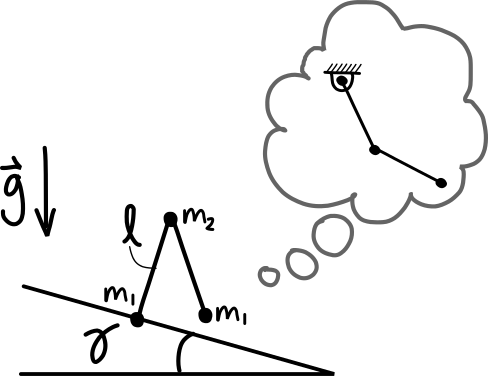
\includegraphics[width=0.5\textwidth]{Figures/SimplestWalkerPendulum}\par
\end{centering}
\caption[Diagram: Simplest Walker Model]{Simplest walker model. This model
consists of only two massless links of length $l$ joined at the hip, with
masses $m_{1}$ and $m_{2}$ at the ends of the links. For certain slopes of the
incline $\gamma$, stable motion is possible.}
\label{fig:SimplestWalkerPendulum}
\end{figure}
%

\subsection*{System description}
\label{sec:SimplestWalkerSystemDescription}

Similar to the rimless wheel model, the locomotive is traverseing an incline
defined by the angle $\gamma$. The leg that is in no-slip contact with the
incline is called the \textit{stance leg} and the other leg is called the
\textit{swing leg}\index{stance leg}\index{swing leg}. The legs are both
massless and have a length $l$. The mass of the hips is $m_{2}$, and the mass
of each foot is $m_{1}$, with $\beta = m_{1} / m_{2} \ll 1$.

% FIGURE
\begin{figure}[h]		% h="here" t="top" b="bottom" p="separate page"
\begin{centering}
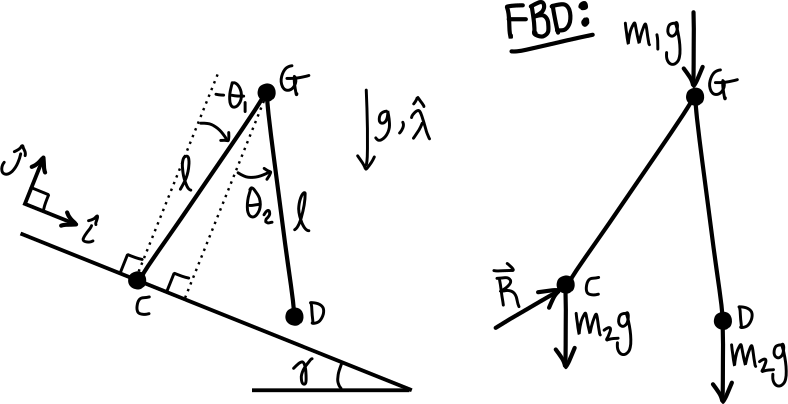
\includegraphics[width=0.8\textwidth]{Figures/SimplestWalkerFBD}\par
\end{centering}
\caption[Diagram: Simplest Walker Free Body Diagram]{Simplest walker free body diagram. The configuration of the model is defined by the rotations $\theta_{1}$ and $\theta_{2}$. Weights act at all three masses, and a ground reaction force acts at the contact point $C$.}
\label{fig:SimplestWalkerFBD}
\end{figure}
%

Unlike the rimless wheel, this system has two degrees of freedom because the
angle between the legs is not fixed. The configuration of the locomotive is
defined by the angles $\theta_1$ and $\theta_2$ and the corresponding angular
speeds $\dot{\theta}_1$ and $\dot{\theta}_2$. Both angles are defined with
respect to the normal of the incline. The free body diagram of the model in
figure \ref{fig:SimplestWalkerFBD} describes this locomotive in more detail.
The forces present in the full system are the weight of each mass and the
reaction force of the incline against the stance leg $\vec{\mathbf{R}}$ (the
vector sum of static friction and normal force). The motion proceeds under the
force of gravity. A free body diagram of the swing leg (not shown) would reveal
a force in the swing leg that is required to maintain the joint constraint at
point $G$. This force is decomposed into two components: tension $T$ along the
swing leg and a force $F$ perpendicular to the swing leg.

\todo{perhaps show an FBD of the swing leg}

\begin{comment}
[chris: in Alan's notes where is F's line of action?]
\end{comment}

\subsection*{Equations of Motion}
\label{sec:SimplestWalkerSystemDescription}

There are six unknowns in this model: the angular acceleration of each degree
of freedom, $\ddot{\theta}_{1}$ and $\ddot{\theta}_{2}$, the tension $T$ and
perpendicular force $F$ in the swing leg, and the two components of the support
force $\vec{\mathbf{R}}$. The system is described by two free body diagrams and
three momentum balances for each diagram. This gives six equations with which
we can solve for all six unknowns. To obtain only the motion of the locomotive
and avoid the support forces and internal forces, only angular momentum balance
is required for each of the two free body diagrams. For the full system free
body diagram, angular momentum balance about $C$ yields

\begin{align}
\Sigma \vM_{/C} &= \vHdot_{/C} \notag \\
(\vr_{G/C} \times m_{1} g  \ul ) + (\vr_{D/C} \times m_{2} g  \ul ) &= (\vr_{G/C} \times m_{1} \va_{G}) + (\vr_{D/C} \times m_{2} \va_{D})
\label{eq:SimplestWalkerAMB1}
\end{align}

where $ \ul $ is directed downward, in the direction of gravity.

Likewise, angular momentum balance of just the swing leg about $G$ yields

\begin{align}
\Sigma \vM_{/G} &= \vHdot_{/G} \notag \\
\vr_{D/G} \times m_{2} g  \ul  &= \vr_{D/G} \times m_{2} \va_{D}
\label{eq:SimplestWalkerAMB2}
\end{align}

To solve these equations, expressions for $\vec{\mathbf{a}}_{G}$ and $\vec{\mathbf{a}}_{D}$ are required.

\begin{align}
\va_{G} &= -\dot{\theta}_{1}^{2} \vr_{G/C} + \ddot{\theta}_{1} \uk \times \vr_{G/C} \\
\va_{D}  &= \va_{G} + \va_{D/G} \notag \\
 &= \va_{G}  -\dot{\theta}_{2}^{2} \vr_{D/G} + \ddot{\theta}_{2} \uk \times \vr_{D/G}
\end{align}

\todo[inline]{I'm not sure the signs for accelerations are correct here, since
theta's are defined positive for cw rotations}

where $\vr_{G/C} = l (- \sin{\theta_{1}} \ui +\cos{\theta_{1}} \uj)$ and
$\vr_{D/G} = l (\sin{\theta_{2}} \ui - \cos{\theta_{2}} \uj)$. The equations
can be greatly simplified if the feet have no mass, $\beta = 0$.


As with the rimless wheel, equations \ref{eq:SimplestWalkerAMB1} and
\ref{eq:SimplestWalkerAMB2} describe the dynamics of the model during the
smooth ``flight''. The solution for the smooth flight motion requires
information about the inelastic collision that occurs between flights. The
instant at which the collision starts is called
\textit{heelstrike}\index{heelstrike}. At heelstrike, point $C$ collides with
the incline and the collision is analyzed by the following equalities across
the collisions

\begin{align}
\vHdot_{/C}^{+} &= \vHdot_{/C}^{-} \notag \\
\vHdot_{/G}^{+} &= \vHdot_{/G}^{-} \notag
\label{eq:SimplestWalkerCollision}
\end{align}

These equations result in expressions that are very similar to equations
\ref{eq:RimlessHPlus} and \ref{eq:RimlessHMinus} for the rimless wheel, except
that this time there are two degrees of freedom to manage. As for the rimless
wheel, the weight of the masses can be ignored in the angular momentum
expressions since the collisions occur so quickly. The coupled differential
equations for $\theta_{1}$ and $\theta_{2}$ and the collision equations are
presented in \cite{garcia97}. \todo{we really don't want to show the derivation
here? I think there needs to be more meat here before we jump into
``stability'',
and our discussion on stability needs to align with our discussion of stability
from previous sections}

\subsection*{Bifurcation}
\label{sec:SimplestWalkerBifurcation}

The equations of motion in this model are actually
\emph{nonlinear}\index{nonlinear}. This means that for certain system
parameters the motion of the locomotive may be chaotic, and so small changes in
initial conditions can result in largely different motions. The simplest walker
model exhibits the \emph{period-doubling}\index{period-doubling} phenomenon as
the angle of the incline $\gamma$ is increased. The period-doubling is captured
in the bifurcation diagram\index{Poincare map} in figure
\ref{fig:SimplestWalkerEigenvalues}.

A bifurcation diagram is a graph in which the value of a state variable of the
model over many periods of the motion is plotted as a function of some
parameter of the model. The natural parameter to use in this case is the angle
of the incline $\gamma$. The vertical axis of this bifurcation diagram holds
the step length for each gait cycle. For small inclines, the step length is
constant for each gait cycle. This is shown in the graph, where there is only
one curve to the left of the dotted vertical line. The point where the curve
splits into two curves is called a \emph{bifurcation point}\index{bifurcation
point}.

\todo[inline]{step length is measured along the incline?}

% FIGURE
\begin{figure}[h]		% h="here" t="top" b="bottom" p="separate page"
\begin{centering}
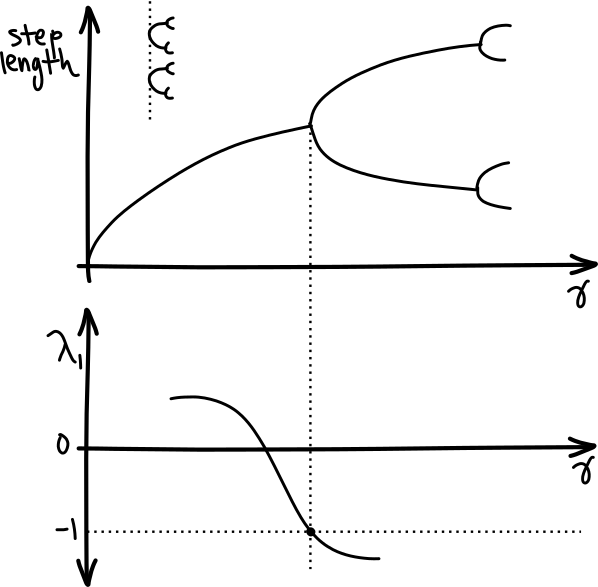
\includegraphics[width=0.6\textwidth]{Figures/SimplestWalkerEigenvalues}\par
\end{centering}
\caption[Plot: Simplest Walker Bifurcation and Eigenvalues]{Simplest walker
bifurcation and eigenvalues. The top plot is a bifurcation diagram that shows
the step length for many gait cycles for a given value of $\gamma$, as $\gamma$
is varied. The bottom plot shows the first eigenvalue of the Jacobian of the
system's Poincare map (map not shown). Eigenvalues of $\lambda = -1$ correspond
to bifurcation points, and consequently, \emph{period-doubling}. Beyond
$\gamma = \gamma^{*}$, the simplest walker executes a limping period-2 gait in
which step length alternates between two values.}
\label{fig:SimplestWalkerEigenvalues}
\end{figure}
%

\todo[inline]{figure: show 0.015 rad, or put in a variable for the gamma value
like gamma star. also, show arrows on the curves to show that they continue
on. Split figure into 4.12(a) and 4.12(b)}

The nonlinear behavior of the model is determined by the Jacobian of the
Poincare map. The first eigenvalue $\lambda$ of this Jacobian follows the curve
presented in figure \ref{fig:SimplestWalkerEigenvalues}. The values of $\gamma$
for which the eigenvalue $\lambda = -1$ are the incline angles at which
bifurcation occurs. After this bifurcation point, the motion is described as
being \textit{period-2}. This means that the step length alternates between two
values between gait cycles. This motion resembles limping, because one leg
takes larger steps than the other.

For $0 < \gamma < \gamma^{*}$ rad, the motion of the simplest walker model is
stable. The fact that such a simple mechanical model of locomotion has stable
solutions without actuation or control hints that the coordinated locomotion is
mostly mechanical. This view is in constrast with a view that states
coordinated locomotion results from muscle action or from neurological control
\cite{garcia97}.

For an in-depth description of the nonlinear behavior of this model, 
refer to Garcia \cite{garcia97}.


\section*{Passive Models of Locomotion}

All the models presented in this chapter and chapter
\ref{sec:ModelingLeggedLocomotion} are very simple. Mass has been concentrated
at the hip or at the foot. More detailed dynamic models of locomotion can be
developed in a somewhat logical fashion. The models can be extended by
including distributed masses for the legs, or perhaps links for the upper body.
For these situations, analytical descriptions quickly become cumbersome. It is
important though to examine if such detailed models add any new information or
provide any additional accuracy. There is an elegance to the ability to make
important conclusions about animal locomotion from the motion of only a few
point masses.


\begin{comment}
-eigenvalues less than one means stability.
-describe poincare/stability
-detail that dHdt vs Hdot only if C is not moving
-didnt talk about the passive nature of the locomotion
\end{comment}
